\section{eo\-Quad\-Op$<$ EOType $>$ Class Template Reference}
\label{classeo_quad_op}\index{eoQuadOp@{eoQuadOp}}
Quad genetic operator: subclasses {\bf eo\-Op}{\rm (p.\,\pageref{classeo_op})}, and defines basically the operator() with two operands, both can be modified.  


{\tt \#include $<$eo\-Op.h$>$}

Inheritance diagram for eo\-Quad\-Op$<$ EOType $>$::\begin{figure}[H]
\begin{center}
\leavevmode
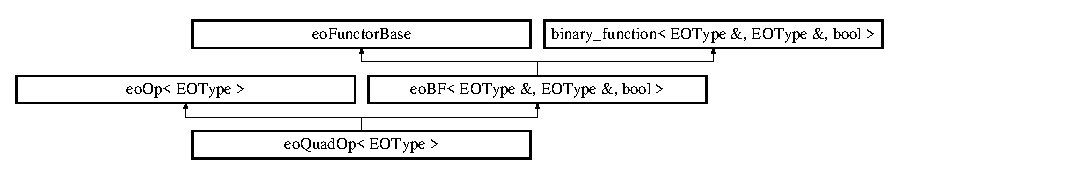
\includegraphics[height=1.90476cm]{classeo_quad_op}
\end{center}
\end{figure}
\subsection*{Public Member Functions}
\begin{CompactItemize}
\item 
{\bf eo\-Quad\-Op} ()\label{classeo_quad_op_a0}

\begin{CompactList}\small\item\em Ctor. \item\end{CompactList}\item 
virtual std::string {\bf class\-Name} () const \label{classeo_quad_op_a1}

\end{CompactItemize}


\subsection{Detailed Description}
\subsubsection*{template$<$class EOType$>$ class eo\-Quad\-Op$<$ EOType $>$}

Quad genetic operator: subclasses {\bf eo\-Op}{\rm (p.\,\pageref{classeo_op})}, and defines basically the operator() with two operands, both can be modified. 

When defining your own, make sure that you return a boolean value indicating that you have changed the content. 



Definition at line 132 of file eo\-Op.h.

The documentation for this class was generated from the following file:\begin{CompactItemize}
\item 
eo\-Op.h\end{CompactItemize}
